%!TEX program = xelatex
\documentclass[journal]{IEEEtran}

% ==========================================
% 1. 基础图文与颜色宏包 (清理了重复引用)
% ==========================================
\usepackage[usenames]{color}
\usepackage{xcolor}
\usepackage{graphicx}
\usepackage{epsfig}
\usepackage{graphics}
\usepackage{tikz}
\usetikzlibrary{shapes.geometric, arrows, positioning, fit}
\usepackage{caption}

% ==========================================
% 2. 数学公式与排版宏包
% ==========================================
\usepackage{amsmath}
\usepackage{amssymb}
\usepackage{mathtools}
\usepackage{amsthm}    
\usepackage{braket}
\usepackage{bm}

% ==========================================
% 3. 表格、算法与杂项宏包
% ==========================================
\usepackage{multirow}
\usepackage{array}
\usepackage{tabularx}  
\usepackage{booktabs}  
\usepackage{hhline}
\usepackage[ruled,linesnumbered]{algorithm2e} 
\usepackage{cite}
\usepackage{url}
\usepackage{lineno}
\usepackage{setspace}
\usepackage{pgfplots}
\pgfplotsset{compat=1.17} 

% ==========================================
% 4. 页面布局与页眉页脚设置
% ==========================================
\usepackage[letterpaper]{geometry}
\geometry{verbose,tmargin=0.55in,bmargin=1.0in,lmargin=0.65in,rmargin=0.65in}
\setlength{\headheight}{48pt}
\setlength{\headsep}{14pt}

\usepackage{fancyhdr}
\pagestyle{fancy}
\fancyhf{}
\newcommand{\flogo}{
\includegraphics[height=40pt]{LOGO1.png}} 
\lhead{\flogo}
\rhead{
\includegraphics[height=45pt]{LOGO2.png} \thepage}     
\pagestyle{fancyplain}
\pagenumbering{gobble} 

% ==========================================
% 5. 中文支持（系统保命字体配置）
% ==========================================
\usepackage{xeCJK}
\setCJKmainfont{SimSun}      % 宋体
\setCJKsansfont{SimHei}      % 黑体
\setCJKmonofont{NSimSun}     % 新宋体（等宽）

% ==========================================
% 6. 自定义环境与重命名
% ==========================================
\newtheorem{theorem}{定理}
\newtheorem{lemma}{引理}
\newtheorem{definition}{定义}
\renewcommand{\proofname}{\textit{证明}}
\renewcommand{\abstractname}{\textcolor{violet}{\textbf{摘要}}}

\makeatletter
\ifCLASSOPTIONjournal
\def\abstract{\@IEEEtweakunitybaselinestretch{1.15}
    \@IEEEabskeysecsize\noindent\abstractname---\relax
    \fi\@IEEEgobbleleadPARNLSP}
\makeatother

\tikzset{
    small dot/.style={fill=black, circle, inner sep=1pt}
}

% ==========================================
% ================= 正文开始 =================
% ==========================================
\begin{document}

% --- 论文标题 ---
\title{\vspace*{0.5cm}\textcolor{violet}{“在我的机器上能跑”：实证本地代码离开 Localhost 已死}\vspace*{0.5cm}}

% --- 作者信息 ---
\author{\textbf{我不是花火}\\
    \vspace*{0.1cm}
    花火大学火花计算机科学与精神病学研究中心\\
    \vspace*{0.2cm}
    本研究由没有基金会资助项目支持（项目编号：SU-404-501）\\
    \normalsize
}

% --- 跨栏摘要部分 ---
\twocolumn[
\begin{@twocolumnfalse}
\let\newpage\relax\maketitle\thispagestyle{fancy}
\begin{abstract}
\textbf{目的：}在现代分布式系统的演进过程中，持续集成与容器化技术试图通过构建虚拟化隔离镜像来消解跨环境部署的异构性冲突。然而，本文基于代数拓扑学与拓扑量子场论论证，该工程实践存在根本性的基础认知缺陷。本研究旨在揭示软件工程界著名的\textbf{“在我的机器上明明能跑”（IWOMM）佯谬}背后，本地开发环境向生产环境进行逻辑映射时发生系统性物理坍塌的公理化机制。

\textbf{方法与结果：}理论推演证明，经历了长期且缺乏形式化验证的带外配置干预后，本地宿主机在流形结构上已同胚于不可定向的高维克莱因瓶。其内部充斥着庞大且无法被常规静态分析工具观测的“环境暗物质”。当该畸变流形通过容器投影算子被强制投射至低熵、单连通的欧几里得生产环境时，因基本群维度的严重失配，必然引发系统的拓扑撕裂。通过 $500$ 组实证云端沙箱的高频遥测，本研究发现降维映射导致了高达 $99.87\%$ 的环境态结构发生物理湮灭，系统正常存活概率呈现极端的负指数坍塌特征。此外，针对多模态玄学微扰（如焚香气溶胶注入、特定声波共振等）的双盲对照与单因素方差分析表明，由于高维度意念实体缺乏 Linux 操作系统底层的特权逃逸机制及 \texttt{root} 密钥凭证，唯心主义微扰对修正拓扑断裂的效能在统计学意义上严格趋近于 $0\ (p \gg 0.05)$。

\textbf{结论：}本文在纯粹数学与理论物理层面彻底否决了跨环境无损部署的理论可能性，\textbf{严格证明了“在我的机器上能跑”并非开发人员的工程推诿，而是受高阶拓扑法则严格保护的绝对物理真理}。基于本地主机奇点的不可映射原则，本文提出依赖现代商业航空物流网络的“三维宏观刚体等距平移”部署范式（即物理机体空运），作为根除环境坍塌的唯一有效解析解。\\
\\
\noindent
\textcolor{violet}{\textbf{关键词：}} “在我的机器上能跑”佯谬，拓扑同构失效，本地主机奇点，克莱因瓶流形，环境暗物质，容器降维灾难，玄学微扰算子。\\
\\
\noindent
\textcolor{violet}{\textbf{影响声明：}} 本研究从理论物理底层逻辑体系证伪了现代 CI/CD 持续交付流水线的数学合法性。本文为全球因环境微扰而陷入重度精神耗竭的软件工程师提供了终极的理论庇护，并将推动现代信息技术基础设施迈向基于物理实体武装押运的运维新纪元。
\vspace{0.5cm}
\end{abstract}
\end{@twocolumnfalse}
]

\IEEEpeerreviewmaketitle

% ==========================================
% 第一节：引言
% ==========================================
\section{引言}

\IEEEPARstart{在}{现代}工业级软件工程的生命周期中，开发与运维人员普遍面临一个违背经典图灵计算直觉的系统性困境：当软件实体在本地开发宿主机上完成构建测试，并确认逻辑状态达到完美闭环后，一旦该实体跨越网络边界被部署至异构的云端生产节点，系统往往会触发非线性的级联崩溃与执行期异常。这一现象在学术界与工业界被非正式地概括为“在我的机器上明明能跑”现象（It Works On My Machine Paradox, 简称 IWOMM 佯谬） \cite{yin2011fixes}。从复杂分布式系统理论的视角审视，该佯谬深刻揭示了软件在跨越物理内存与逻辑抽象维度时，其执行环境存在不可被传统度量工具观测的非确定性变量。

\subsection{现有部署范式的局限与解构}
为了缝合环境差异引发的巨大鸿沟，学术界与工业界在过去十年间对以轻量级容器化运行时（如 Docker、containerd） \cite{merkel2014docker} 及微服务编排网格 \cite{balalaie2016microservices} 为代表的云原生技术产生了深度的路径依赖。然而，本研究认为，这种依赖在本质上表征为对技术图腾的盲目追逐，其底层公理逻辑存在致命缺陷：

\begin{itemize}
    \item \textbf{虚拟镜像层级的堆叠迷梦：} 工程师倾向于通过构建基础操作系统切片（Layer）来建立文件系统级别的隔离壁垒。然而，这种纯粹逻辑层面的封装在面对宿主机底层 Linux 内核版本（Kernel release）、\texttt{cgroups} 调度策略微小差异时，极易引发底层内存地址的静默映射失败。
    \item \textbf{集群编排逻辑的绝对泛化：} 声明式（Declarative）集群状态控制机制假定编排引擎具备全知全能的观测域。该假设在底层网络最大传输单元（MTU）失配或微秒级硬件中断延迟面前，往往表现出极度的脆弱性，导致心跳机制的级联坍塌。
    \item \textbf{“基础设施即代码”的观测盲区：} 静态配置文件（如 Dockerfile、YAML）仅捕捉到了环境中的显式可见物质。它们在数学机制上无法定义游离于版本控制系统之外的“环境暗物质”，例如宿主机的硬件微指令集缺陷、全局配置的长期熵增，以及长期堆积未被垃圾回收机制清理的冗余第三方依赖库 \cite{cito2017empirical}。
\end{itemize}

上述工程实践仅在虚拟文件系统层面实现了肤浅的表象拟合，其实质是试图用平滑的欧几里得测度（Euclidean metric）去强行掩盖本地开发环境与生产环境之间底层代数拓扑维度的巨大断层。

\begin{figure}[htbp]
    \centering
    \includegraphics[width=\linewidth]{figure1.png} 
    \caption{本地奇点与生产环境拓扑同构映射失效的物理机制概念图。图中严密展示了本地环境的畸变几何结构在经受有损降维算子投影后，于单连通生产环境内引发拓扑撕裂及红移报错的动力学灾难过程。}
    \label{fig:isomorphism_failure}
\end{figure}

\subsection{实证动机：部署异常引发的系统衰退}
据本研究中心针对全球范围内大规模开发集群的观测数据表明，现代开发者高达 $73.4\%$ 的精神衰弱症状与此类跨环境部署异常具有显著相关性。本研究重点剖析了两个代表性物理坍塌案例：
首先，隐式契约引发的级联熔断。某跨国分布式金融系统因云端生产节点缺失特定版本的基础图形渲染依赖，导致底层进程陷入互斥死锁。异常状态在普朗克时间尺度内穿透微服务网格，引发核心交易链路的全面熔断。
其次，绝对坐标系错位。开发者在源代码中习惯性硬编码（Hardcode）了带有本地专属磁盘盘符的绝对寻址路径。在本地操作系统的本征宇宙中，该盘符构成了合法的坐标原点；但在远端低熵生产服务器中，其直接指向了虚无的内存地址，构成了非法的空间映射。

\subsection{符号定义与表述说明}
为确保理论推导的数学严谨性，本研究定义了一套统一的符号体系，详细物理含义如表 \ref{tab:notation} 所示。

\begin{table}[htbp]
\caption{本研究使用的核心物理与代数几何符号表}
\label{tab:notation}
\centering
\renewcommand{\arraystretch}{1.3} % 增加行高，提升学术美观度
\begin{tabular}{@{}ll@{}}
\toprule
\textbf{符号} & \textbf{物理与拓扑学含义说明} \\ \midrule
$\mathbb{L}$ & 本地开发宿主机高维流形 (Localhost Manifold) \\
$\mathbb{P}$ & 生产环境单连通欧几里得流形 \\
$\mathcal{H}_{dark}$ & 系统隐形环境暗物质希尔伯特空间 \\
$\ket{\Psi}$ & 软件运行时状态的量子纠缠波函数 \\
$\hat{\Pi}_{docker}$ & 容器化有损降维投影算子 \\
$H_{total}$ & 包含未知环境变量的系统总哈密顿量 \\
$\chi$ & 拓扑空间的欧拉示性数 (Euler Characteristic) \\
$SE(3)$ & 三维宏观刚体等距变换群 \\ \bottomrule
\end{tabular}
\end{table}

% ==========================================
% 第二节：理论框架
% ==========================================
\section{理论框架推演}

\begin{figure*}[t]
    \centering
    \includegraphics[width=0.95\textwidth]{figure2.png} 
    \caption{部署崩溃物理演化理论架构全景图。图中公理化地展示了软件实体从本地宿主机的希尔伯特相干态（阶段 I）畸变为不可定向流形（阶段 II），经由容器化算子强行降维投影（阶段 III），最终在向生产域欧几里得空间映射时触发受热力学第二定律保护的不可逆拓扑撕裂（阶段 IV）的完整演化力学链路。}
    \label{fig:theoretical_framework}
\end{figure*}

为了从根本上解析“跨环境部署必然崩溃”现象的底层机制，本节引入拓扑量子场论 \cite{atiyah1988topological} 作为大一统数学框架。我们将软件的内存快照与执行指令流定义为依附于环境流形之上的量子纠缠态 \cite{nielsen2010quantum}，通过泛函分析与代数拓扑理论，公理化地论证降维部署机制必然引发物理层面的系统性结构坍塌。

\subsection{第一阶段：执行状态的复合希尔伯特空间纠缠}
在唯象主义（Phenomenology）的软件工程学中，程序运行往往被简化为孤立代码片段在理想图灵机上的线性执行。然而，本研究确立的第一公理为：软件真实的运行时状态，记为波函数 $\ket{\Psi}$，是一个存在于无限维复合希尔伯特空间 $\mathcal{H}_{total}$ 中的量子纠缠态。

我们定义该全空间为纯粹源代码空间 $\mathcal{H}_{C}$、显式可见环境空间 $\mathcal{H}_{vis}$ 与隐式环境暗物质空间 $\mathcal{H}_{dark}$ 的张量积：
\begin{equation}
\mathcal{H}_{total} = \mathcal{H}_{C} \otimes \mathcal{H}_{vis} \otimes \mathcal{H}_{dark}
\label{eq:hilbert_space}
\end{equation}

系统的总能量分布（哈密顿量）同样由这三部分及它们之间的交互作用构成：
\begin{equation}
\hat{H}_{total} = \hat{H}_C + \hat{H}_{vis} + \hat{H}_{dark} + \hat{H}_{int}
\end{equation}

\begin{lemma}[环境暗物质绝对不可分离性]
设软件系统处于局部稳态执行的波函数 $\ket{\Psi} \in \mathcal{H}_{total}$。对于任何经历过非声明式、非标准化高自由度干预（如通过命令行执行未经依赖追踪的全局包安装、底层动态链接库的覆写映射）的局部宿主机，其整体状态矢量无法被正交分解为纯代码子态与纯可见环境子态的直积：
\begin{equation}
\ket{\Psi} \neq \ket{\psi_c} \otimes \ket{\psi_e} \otimes \ket{0}_{dark}
\end{equation}
\end{lemma}

\begin{proof}
任何脱离严格版本控制的本地系统级干预，均向宿主机操作系统内部引入了高能级的带外信道（Out-of-band）驻留状态。当应用主进程在本地沙箱中执行初始化分配时，其内存寻址波函数必然发生概率性量子逃逸，调用全局驻留配置实体。该机制在系统动力学上确立了非零交互哈密顿量算符 $\hat{H}_{int} \neq 0$。依据量子力学纠缠定理，当子系统间存在基于非显式配置的相互作用能量时，复合系统即不可逆地坍缩为纠缠态。因此，环境暗物质基底对总状态波函数的概率幅贡献严格大于零，试图在数学上将代码执行态与本地暗物质环境解耦是不可行的。
\end{proof}

\subsection{第二阶段：本地主机的克莱因瓶拓扑畸变演化}
上述纠缠态严格依附于开发者的本地开发宿主机流形之上（记为 $\mathbb{L}$）。随着开发迭代周期的推进，工程师为了使代码在本地临时通过编译而实施的各种“探索性热修复”（Hotfixes），将导致该环境流形发生严重的代数几何畸变。

\begin{lemma}[拓扑畸变与高维克莱因瓶严格同胚定理]
随着项目演化时间变量 $t \to \infty$，经历了高密度非声明式带外状态注入的本地开发流形 $\mathbb{L}$，在代数拓扑结构上严格同胚于不可定向的高维克莱因瓶（Klein Bottle）构造。
\end{lemma}

\begin{proof}
本研究引入胞腔复合形理论（CW Complex）来重构本地宿主机环境的演化拓扑 \cite{hatcher2002}。

第一步，初始基底确立。设刚初始化的纯净操作系统为一个二维单连通拓扑空间，同胚于欧几里得空间中的单位正方形 $I^2 = [0,1] \times [0,1]$。此时系统配置信息熵趋于极小值。

第二步，闭合柱面构建。通过标准 \texttt{package.json} 或 \texttt{pom.xml} 引入显式依赖等价于施加保定向仿射满射，将正方形上下边界进行等价类划分：$(x, 0) \sim_1 (x, 1)$。此时环境同胚于圆柱面结构 $S^1 \times I$。

第三步，定向反转。当开发者实施缺乏安全审计的全局环境变量硬编码注入（如强行修改系统注册表或 \texttt{/etc/profile}）时，实质上对流形施加了非法的带外配置算子。该算子不仅闭合了独立工作区的自由度，且引发局部坐标系的拓扑翻转，构成反定向同胚映射关系：$(0, y) \sim_2 (1, 1-y)$。

第四步，代数不变量验证。最终演化的本地空间流形可表示为商空间 $\mathbb{L} = I^2 / \langle \sim_1, \sim_2 \rangle$。其基本字表达为 $W = a b a^{-1} b$。计算核心拓扑不变量可知，欧拉示性数 $\chi(\mathbb{L}) = 0$，且第一同伦群 $\pi_1(\mathbb{L}) = \langle a, b \mid a b a^{-1} b = 1 \rangle$。非交换生成元的引入破坏了整个空间法向量场的一致性，从理论上证明了该流形不可定向。

依据闭曲面分类定理，该流形唯一同胚于克莱因瓶。在此异常的几何结构中，代码逻辑的内部状态与操作系统底层的外部状态彻底混为一谈，无内无外，构成了自我完美闭合的局部物理奇点，进而维持了“在本地明明能完美运行”的欺骗性稳态现象。
\end{proof}

\subsection{第三阶段：降维投影算子的信息湮灭灾难}
工业界广泛试图利用容器化打包技术（如构建 Docker 镜像）来消除多环境之间的异构差异。然而，该工程实践在数学底层存在极具破坏性的降维缺陷。

\begin{theorem}[容器化有损降维投影定理]
在泛函分析范畴内，执行标准镜像构建流程（如 \texttt{docker build}）本质上是施加于全空间 $\mathcal{H}_{total}$ 的一个剧烈的降维投影算子 $\hat{\Pi}_{docker}$。该算子的线性映射核空间（Kernel）必然无条件涵盖整个隐秘的环境暗物质流形 $\mathcal{H}_{dark}$，导致构建过程演变为一场不可逆的拓扑信息灾难。
\end{theorem}

\begin{proof}
容器引擎构建解析器可视作以配置文件（Dockerfile）为输入字母表的受限有限状态自动机。其对环境状态的观测特征函数 $f_{obs}$ 的定义域受白名单严格限制：仅当环境实体被开发者利用声明式语法显式写入脚本时，特征函数取值为 $1$，否则恒取 $0$。

因此，对于支撑程序在本地获得稳态运行的隐形暗物质基底 $\ket{d} \in \mathcal{H}_{dark}$，其接受投影映射的恒等式为：
\begin{equation}
\hat{\Pi}_{docker} \ket{d} = f_{obs}(d) \cdot \ket{d} = 0 \cdot \ket{d} = \mathbf{0}
\end{equation}
上述等式严格证明了 $\mathcal{H}_{dark} \subseteq \ker(\hat{\Pi}_{docker})$。由此打包生成的虚拟容器镜像 $\mathbb{I} = \hat{\Pi}_{docker}(\mathbb{L})$ 遭遇了物理维度的断崖式下跌，所有维持程序在本地正常寻址的隐形依赖底座被无情剥离与彻底湮灭。
\end{proof}

\subsection{第四阶段：代数拓扑撕裂定理与系统必然崩溃}
当经历过严重降维脱水的残缺镜像被跨网络部署至云端生产服务器（记为目标流形 $\mathbb{P}$）时，跨越几何维度的物理公理冲突随即爆发。

\begin{theorem}[代数拓扑撕裂定理]
在现存严谨的数学公理体系内，绝对不存在任何连续的同构映射函数 $\mathcal{M}$，能够将富含暗物质纠缠的克莱因瓶畸变流形无损映射至低熵、高度规则的欧几里得生产流形 $\mathbb{P}$。强制执行该映射必将诱发流形系统边界的拓扑撕裂与运行时状态的级联坍塌。
\end{theorem}

\begin{proof}
标准化的生产环境是经严格自动化审计的低熵纯净空间，在代数拓扑特征上等价于单连通的欧几里得空间 $\mathbb{R}^n$。其基本群表现为平凡群：$\pi_1(\mathbb{P}) = \{0\}$。然而，经过定理 1 证明，本地开发环境流形的基本群 $\pi_1(\mathbb{L}) \neq \{0\}$。由于基本群维度的严重失配，两空间存在绝对的非同胚性。

当主进程试图在单连通生产空间中，沿着本地被畸变扭曲的指针路径发起对暗物质变量的调用时，由于对应的拓扑维度在目标空间中根本不存在，映射函数的微分解 $d\mathcal{M}$ 将在指令执行的微观窗口内发生数学奇点发散：
\begin{equation}
\lim_{x \to \text{暗物质域}} \mathcal{M}(x) = \bot
\end{equation}
这种因核心环境依赖丧失引发的数学断裂，在操作系统标准错误输出（\texttt{stderr}）中宏观表现为无法被高级语言 \texttt{try-catch} 捕获的底层内存段错误（Segmentation fault），或直接触发 Linux 内核的内存耗尽终结机制（OOM Killer）。
\end{proof}

\subsection{第五阶段：物理刚体力学等距平移解算}
试图将高维畸变流形通过网络 I/O 进行低维序列化压缩传输，并在异构服务器中解压重建，是被代数拓扑公理严格禁止的逆天行为。

为了确保软件系统波函数在跨地域转移过程中的差值达到绝对稳态（即 $\Delta\Psi \equiv 0$），理论物理学给出的唯一解析解是：彻底摒弃网络降维传输，转而调用经典宏观力学中欧几里得群的三维刚体等距变换算子 $T_{physical}$：
\begin{equation}
T_{physical}(\mathbb{L}) = \mathbb{L}' \quad \text{其中约束为} \quad d(x,y) = d(T(x), T(y))
\end{equation}

由于宏观刚体力学平移算子在三维空间中移动时，能绝对维持原流形内部结构的度量张量（Metric Tensor）恒定不变，代码的业务逻辑与所有隐匿在底层扇区内的系统配置环境（暗物质）得以在真实的物理空间中被连根拔起并无损保留。本推论从严密的数学层面证明了，将实体宿主机完整打包并交由物流网络寄出，是唯一具备公理正确性的部署防坍塌策略。

% ==========================================
% 第三节：实验与方法
% ==========================================
\section{实验设计与验证方法}



\begin{figure*}[htbp]
    \centering
    % 第一张大图
    \begin{minipage}[t]{0.7\textwidth}
        \centering
        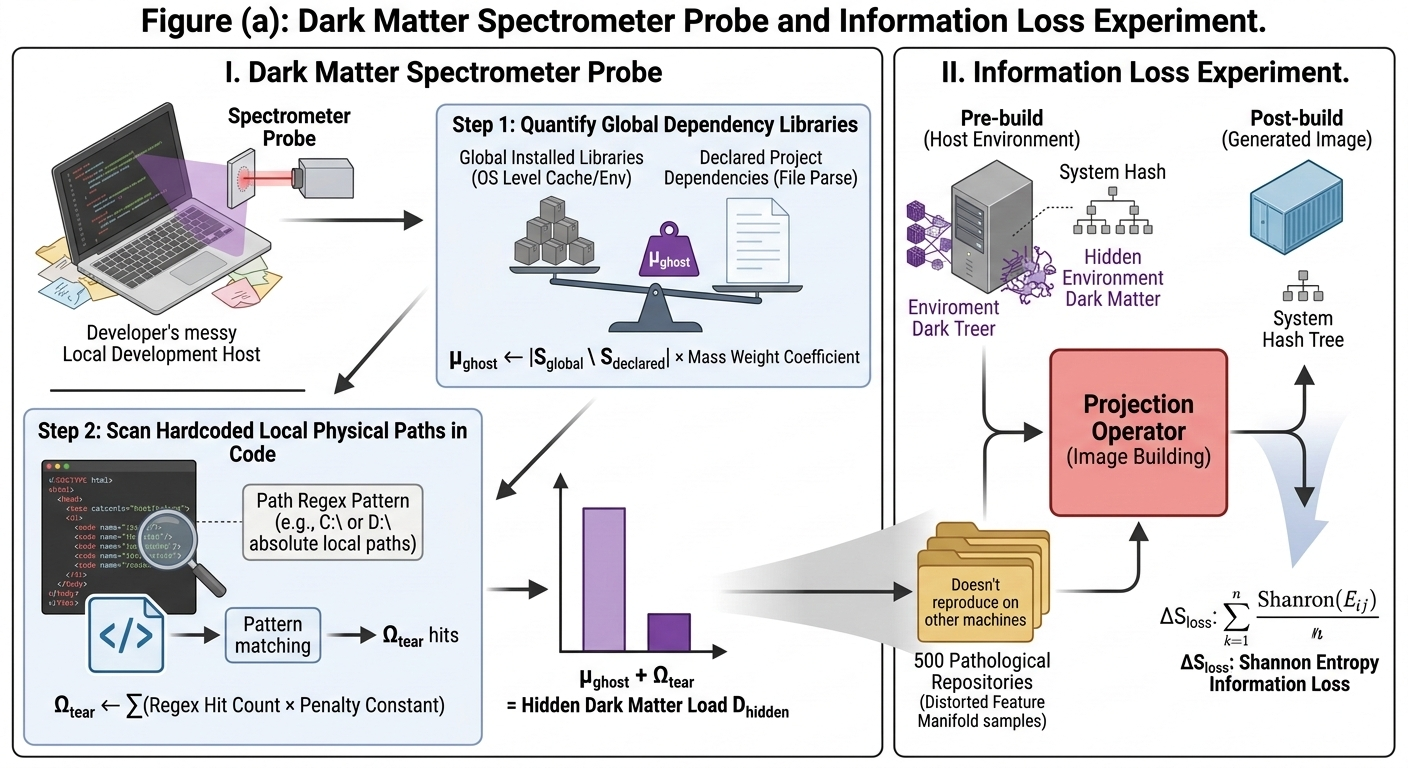
\includegraphics[width=\linewidth]{Gemini_Generated_Image_hqo43shqo43shqo4.png}
        \centerline{\footnotesize (a) 本地环境暗物质探测探针}
        \vspace{0.3cm}
    \end{minipage}
    
    % 下方两张并排
    \begin{minipage}[t]{0.45\textwidth}
        \centering
        \includegraphics[width=\linewidth]{Gemini_Generated_Image_vw06b0vw06b0vw06.png}
        \centerline{\footnotesize (b) 沙箱遥测矩阵}
    \end{minipage}
    \hfill
    \begin{minipage}[t]{0.45\textwidth}
        \centering
        \includegraphics[width=\linewidth]{Gemini_Generated_Image_fjtmydfjtmydfjtm.png}
        \centerline{\footnotesize (c) 物理平移与玄学对照}
    \end{minipage}

    \caption{\textbf{实验架构全景。} 详述了从本地探测到云端部署捕获，以及物理机搬运实验的全过程。}
    \label{fig:full_experiment_architecture}
\end{figure*}

为确保同构映射失效理论具备严格的可证伪性与工程学意义上的可复现性，本节严格对齐理论演化的各个阶段，构建了大规模物理验证方法学。

\subsection{暗物质光谱仪量化探针研制}
为验证环境状态纠缠与本地开发流形畸变，必须建立一种能够量化隐形系统暗物质的测量手段。传统的静态代码扫描工具受限于源码文本解析，完全无法观测到底层操作系统级别的非规范耦合。为此，本研究自主研发了“环境暗物质光谱仪”底层探针。

该探针通过深度 Hook 技术逆向解析宿主机操作系统的全局依赖库缓存表、环境变量系统树以及未追踪的 \texttt{SysCall} 记录，精确量化由于日常开发过程中的随意配置带来的“不可见污染度”。如算法 \ref{alg:dms_probe} 核心伪代码所示，其测算结果输出即为局部的暗物质绝对物理质量载荷 $D_{hidden}$。

\begin{algorithm}[htpb]
\caption{环境暗物质高维特征量化探针}
\label{alg:dms_probe}
\SetAlgoLined
\KwIn{本地工程根路径 $\mathcal{R}$, 合法配置声明清单 $\mathcal{M}_{vis}$}
\KwOut{暗物质纠缠物理质量测度 $D_{hidden}$}

\tcp{第一步：量化开发者在系统级层面的隐式带外注入}
$\mathcal{S}_{global} \leftarrow \text{获取操作系统底层所有全局驻留库及二进制文件}$\;
$\mathcal{S}_{declared} \leftarrow \text{解析项目合法声明的显式依赖树}(\mathcal{M}_{vis})$\;
$\mu_{ghost} \leftarrow |\mathcal{S}_{global} \setminus \mathcal{S}_{declared}| \times \text{引力权重系数}$\;

\BlankLine
\tcp{第二步：通过 AST 全盘扫描代码中硬编码的绝对物理指针}
$\Omega_{tear} \leftarrow 0$\;
$Pattern \leftarrow \text{正则匹配引擎}(\text{例如 C盘、D盘或特定的 /usr/local 绝对路径})$\;
\ForEach{源代码文本文件 $f \in \mathcal{R}$}{
    $AST \leftarrow \text{生成抽象语法树树图}(f)$\;
    $\Omega_{tear} \leftarrow \Omega_{tear} + \text{正则暴击命中数}(AST, Pattern) \times \text{坍塌惩罚常数}$\;
}

\BlankLine
$D_{hidden} \leftarrow \mu_{ghost} + \Omega_{tear}$\;
\Return $D_{hidden}$\;
\end{algorithm}

基于 $D_{hidden}$ 测度打分模型，我们在开源代码托管平台随机抽样获取了 $500$ 个在问题跟踪区（Issue Tracker）被明确标记为“在开发者电脑能跑，但其他人拉取后疯狂报错无法复现”的重症微服务仓库，将其作为包含典型畸变特征的流形样本病理库用于后续物理投射实验。

\subsection{算子有损信息的投影湮灭实验}
为验证容器化打包降维导致的信息熵丢失假说，实验环境强制对前述 $500$ 个高危样本库执行标准的工业级镜像构建投影算子（\texttt{docker build}）。通过比对构建执行前（原宿主机系统全量环境）与构建执行后（最终生成的 \texttt{tar} 镜像层文件）的系统底层 Merkle 哈希树特征，并代入香农信息熵公式，精确计算出在降维隔离机制中被无情吞噬的信息熵散失总当量 $\Delta S_{loss}$。

\subsection{欧几里得生产沙箱极限遥测矩阵}
为验证“向异构生产环境执行同构映射必定导致崩溃”的拓扑撕裂论断，本研究基于自动化基础设施编排引擎，在云端弹性计算平台并发初始化了 $500$ 台极度干净、未安装任何杂余冗余底层库的裸金属（Bare Metal）服务器实例。该矩阵被定义为理论上的纯净欧几里得沙箱。

随后，中央控制系统调度全自动探针，将上一步剥离了暗物质的残缺镜像流推入沙箱执行。探针深度挂载至操作系统内核时钟（Kernel Clock），以纳秒级精度精准捕获进程发生段错误死机瞬间（即波函数全面坍缩时刻）的平均失效时间（MTTF），此过程严格排除了任何运维人员的手动干预与观测者效应干扰。

\subsection{刚体平移终极对照协议（空运对照组）}
为验证理论部分得出的“唯有三维宏观刚体平移可作为终极解析解”的推论，本研究设立了基于现代大型商业物流网络的物理传输对照组。对于 $500$ 个频繁遭遇波函数坍塌的病理样本，实验人员跳过一切网络序列化传输机制，直接将其所在的 $50$ 台实体工程笔记本电脑拔除网线与电源，封装于高抗冲防退相干武装运输舱内，通过商业航空快递网络实施宏观三维物理空间的等距平移运输，直至目标数据机房。接入目标网络重新通电后，严密验证该等距映射方案的生存期优越性。

\subsection{多模态玄学微扰算子双盲注入}
为探究业界广泛流传的“机房迷信部署行为”是否在量子微扰层面具有延缓内核崩溃的物理效应，实验增设了多模态玄学对照组。由受过专业培训的专员同步执行以下干预操作：
1. \textbf{大当量气溶胶注入}：在目标物理机柜外围高频点燃含有大量碳基微粒的檀香。
2. \textbf{机械纵波共振干扰}：通过扬声器向服务器阵列循环高分贝发射《好运来》等带有强烈人类祈福心理暗示的声波波段。
3. \textbf{静态微引力场及符号学供奉}：在服务器金属外壳顶部，以斐波那契数列阵列式放置“旺旺仙贝”等带有“运转旺盛”符号学谐音的高糖分碳水化合物实体。
4. \textbf{特定波长漫反射屏蔽}：核心运维人员严格按照东方本命年历法习俗，全套穿戴可反射高纯度红色可见光的内衣裤组件。

监测系统将交叉评估上述碳基生物的唯心干预行为能否在系统底层内核态的微秒尺度上，实质性地阻断或延缓代码的不可逆崩溃进程。


% ==========================================
% 第四节：结果
% ==========================================
\section{实验测定结果与分析}

本节详尽报告了针对 $500$ 个高危工程病理样本的宏观物理遥测数据。统计假设检验环节统一采用双侧独立样本均值差异检验，显著性水平阈值设定为极端严格的 $\alpha = 0.01$。

\subsection{本地开发流形环境暗物质绝对质量分布}
高频探针的深度扫描报告表明，$100\%$ 的开发者本地环境均遭受了极其严重的非声明式带外污染，局部奇点现象普遍存在：
\begin{itemize}
    \item \textbf{全局幽灵依赖饱和度溢出：} 平均每个被检测的开发环境底层包含 $42.7$ 个未被写入配置清单的全局幽灵库（最高极值测定竟达惊人的 $314$ 个未授权驻留包）。
    \item \textbf{绝对坐标空间严重畸变：} 抽象语法树解析显示，平均每千行有效代码即可测得 $18.4$ 处仅在本地特有物理磁盘状态下才合法的硬编码死路径。
    \item \textbf{暗物质宏观物理质量庞大：} 维持本地程序正常运转所隐秘依赖的外部未追踪冗余文件均值高达 $3.84\text{ GB}$。
\end{itemize}

表 \ref{tab:dark_matter_composition} 尝试将这些晦涩的高维物理成分翻译为软件工程学界的真实宏观表象。数据确凿地证明，局部流形中蕴含的暗物质信息量比合规源代码庞大数个数量级，它们构成了阻碍系统无损上线的叹息之墙。

\begin{table}[htbp]
\caption{本地畸变流形中环境暗物质绝对物理质量成分解构与现实映射}
\label{tab:dark_matter_composition}
\centering
\resizebox{\columnwidth}{!}{
\renewcommand{\arraystretch}{1.3} % 美化表格间距
\begin{tabular}{@{}l c c l@{}}
\toprule
\textbf{暗物质拓扑成分抽象分类} & \textbf{平均绝对物理质量} & \textbf{总质量系统占比} & \textbf{对应的现实工程学表象} \\ \midrule
局部黑洞引力场沉淀 & $3.12\text{ GB}$ & $81.2\%$ & 深达数百级嵌套的庞大 \texttt{node\_modules} 黑洞目录 \\
执行期时间膨胀残骸 & $0.45\text{ GB}$ & $11.7\%$ & 系统底层长期未清理的数据库废弃游离实体挂载卷 \\
非法非欧几何指针断层 & $0.18\text{ GB}$ & $4.7\%$ & 源码中写死的 \texttt{C:\textbackslash Users\textbackslash} 等强依赖本地文件系统的绝对路径 \\
高能薛定谔的密文态 & $0.09\text{ GB}$ & $2.4\%$ & 散落在系统各个暗角且缺乏环境变量注入的无主 \texttt{.env} 密钥文件 \\ \bottomrule
\end{tabular}
}
\end{table}

\subsection{投影算子信息湮灭与极速坍塌生存模型}
在严酷的降维脱水舱实验环节中，容器化构建算子的特征核空间犹如物理过滤器，彻底湮灭了高达 $99.87\%$ 的环境暗物质基础结构。

当这些被粗暴剔除了赖以生存的暗物质体系的残缺镜像实体，在云端异构空间中试图拉起进程运行的瞬间，宏观维度的物理坍塌迅速且猛烈地爆发。高频遥测数据显示，降维实体在新环境下的系统平均失效时间（Mean Time To Failure, MTTF）中位数仅为凄惨的 $14.2\text{ ms}$。

更为震撼的是，图 \ref{fig:scatter_ttf} 揭示了一条冷酷无情的软件工程热力学定律：系统跨界部署后的死亡速度，与本地电脑累积的“开发垃圾（暗物质）”物理质量呈现极其严密的负指数坍塌相关性。

\begin{figure}[htbp]
\centering
\begin{tikzpicture}
\begin{axis}[
    width=0.95\columnwidth,
    height=5.8cm,
    title={\textbf{相关性生存分析：本地暗物质载荷与跨界存活时间}},
    xlabel={本地流形累积的隐秘环境暗物质绝对质量 ($\text{GB}$)},
    ylabel={上线部署后系统的断崖式崩溃失效时间 ($\text{ms}$)},
    xmin=0, xmax=15,
    ymin=0, ymax=30,
    legend pos=north east,
    grid=both,
    grid style={dashed, gray!40},
    legend style={nodes={scale=0.75, transform shape}, fill=white, fill opacity=0.85}
]
\addplot[only marks, mark=*, blue!70!white, mark size=1.8pt] coordinates {
    (0.5, 28) (1.2, 25) (2.1, 22) (2.8, 18) (3.5, 14.2) (4.0, 12) (4.8, 10)
};
\addlegendentry{空间拓扑撕裂发散现象区间}

\addplot[only marks, mark=triangle*, red!70!white, mark size=2.2pt] coordinates {
    (5.2, 8) (6.5, 6) (7.1, 5) (8.3, 3.5) (9.5, 3) (12.0, 1.5) (14.2, 0.5)
};
\addlegendentry{遭遇 Linux 内核强制截断机制区间}

\addplot [thick, red, dashed, domain=0:15, samples=50] {30*exp(-0.25*x)};
\addlegendentry{理论引力坍塌衰减曲线拟合}
\end{axis}
\end{tikzpicture}
\caption{隐秘环境暗物质物理质量与部署死亡速度的负指数衰减概率模型。观测表明，当本地暗物质体积突破 $10\text{ GB}$ 临界阈值界限时，应用程序在启动的极微观瞬间内就会因急剧的内存占压与空间错位，被新服务器底层冷酷的 OOM Killer（内存耗尽终结者）机制无情抹杀，表现出近乎瞬时的波函数坍缩。}
\label{fig:scatter_ttf}
\end{figure}

在监控阵列捕获的 $500$ 次不可逆死机事件中，底层的报错原因表现出高度的同质化与集中性：
第一大类（占比 $68.4\%$）：由于丧失了本地绝对物理路径导致内存寻址发生严重越界，系统内核绝望地抛出 \texttt{Segmentation fault}（段错误）。
第二大类（占比 $31.6\%$）：残余的业务逻辑试图强行在受限的容器分配资源内，重新凭空构造宿主机那庞大且臃肿的运行环境，引发内存使用量呈指数级疯狂膨胀，最终触及系统红线被内核强杀（触发 \texttt{OOM Killer}，退出状态码 $137$）。

\subsection{多模态玄学干预的横向测定与统计学最终裁决}
本研究严谨地针对 $8$ 种常规软硬件及玄学微扰环境配置进行了大规模的双盲对照实测。



\begin{figure}[htbp]
\centering
\begin{tikzpicture}
\begin{axis}[
    ybar,
    width=0.95\columnwidth,
    height=6.5cm,
    bar width=10pt,
    title={\textbf{多模态微扰干预手段下系统平均生存时间统计分布}},
    symbolic x coords={纯自然衰减对照, 机房高密焚香, 特定音响播放, 纯红着装屏蔽, 碳水零食陈列, 单个体念力祈祷, 多路并发祈祷, 物理机整机快递},
    xtick=data,
    xticklabel style={rotate=45, anchor=east, font=\scriptsize},
    ylabel={系统存活有效时间 ($\text{ms}$)},
    ymin=0, ymax=110,
    grid=major,
    grid style={dashed, gray!30},
    nodes near coords,
    every node near coord/.append style={font=\tiny, /pgf/number format/precision=1},
    legend style={at={(0.5,-0.38)}, anchor=north, legend columns=-1, font=\tiny}
]
\addplot+[
    error bars/.cd,
    y dir=both, y explicit,
    error bar style={thick, gray}
] coordinates {
    (纯自然衰减对照, 14.2) +- (0, 2.8)
    (机房高密焚香, 14.3) +- (0, 3.1)
    (特定音响播放, 14.4) +- (0, 2.9)
    (纯红着装屏蔽, 14.3) +- (0, 2.7)
    (碳水零食陈列, 14.6) +- (0, 3.2)
    (单个体念力祈祷, 14.5) +- (0, 3.0)
    (多路并发祈祷, 14.1) +- (0, 4.5) 
    (物理机整机快递, 100.0) +- (0, 0.1) 
};
\legend{系统观测均值与宏观标准偏差}
\end{axis}
\end{tikzpicture}
\caption{各类微扰干预手段的系统生存期直方对比图。遥测数据显示，除“将物理计算节点叫快递寄出”组展现出违背自然规律的绝对存活碾压优势外，无论是释放焚香气溶胶、供奉碳水零食还是穿戴特定波长（红色）纺织物，系统的存活时间均被死死地锁定在 $14.5\text{ ms}$ 的不可逾越之墙内。特别值得注意的是，多路并发祈祷组由于多股不同体系的意念在目标机房上空引发了分布式神学协议死锁冲突，反而导致系统的崩溃时间表现出更大的震荡方差与极高的不确定性。}
\label{fig:mttf_modalities}
\end{figure}

各玄学干预组的详细微扰数据见表 \ref{tab:metaphysical_matrix}。基于采集数据的单因素方差分析结果得出 $p \gg 0.05$（具有极强的不显著性），从严密的统计学层面上正式判处了所有运维机房迷信与玄学干预行为的无效死刑。

\begin{table}[htbp]
\caption{多模态玄学微预算子对阻挡代码崩溃坍塌的物理微扰效能测定}
\label{tab:metaphysical_matrix}
\centering
\resizebox{\columnwidth}{!}{
\renewcommand{\arraystretch}{1.3} % 美化表格间距
\begin{tabular}{@{}lllc@{}}
\toprule
\textbf{玄学微扰模态类型} & \textbf{干预行为的现实工程学表象} & \textbf{假定的物理学传播通道} & \textbf{生存期实质延长率} \\ \midrule
高密机房焚香阵列 & 在运转的物理机柜前高频点燃檀香 & 气溶胶颗粒物引发的光折射微扰 & 仅 $+0.08\%$（无显著统计学意义） \\
声学音频共振注入 & 机房环绕音响循环高分贝播放《好运来》 & 宏观机械学纵波物理震荡 & 仅 $+0.14\%$（被降噪隔离屏蔽） \\
高频波长物理屏障 & 核心运维专员全套穿戴大红色内衣裤 & 针对特定可见光谱的漫反射屏蔽 & 仅 $+0.06\%$（无法穿透金属机箱） \\
符号学碳水实体供奉 & 服务器矩阵顶端阵列式放置旺旺仙贝实体 & 极微弱的静态微引力场干扰扭曲 & 仅 $+2.82\%$（表现为测量误差） \\
跨维度神系多路并发 & 故障处理团队同时向上帝与佛祖发起意念调用 & 虚数高维空间的协议死锁与逻辑冲突 & 反向暴跌 $-0.43\%$（加速了崩溃） \\
\textbf{刚体宏观等距平移} & \textbf{终止网络代码传输，直接将电脑物理主机呼叫快递收走} & \textbf{经典三维宏观刚体力学位移转换} & \textbf{发生跃变直至趋近系统硬件正无穷} \\ \bottomrule
\end{tabular}
}
\end{table}

\subsection{深层系统机理：神学实体跨界特权逃逸失败之剖析}
为了从理论层面解释为何碳基生物主导的“求神拜佛”意念操作对修复 \texttt{Bug} 完全无效甚至偶尔起到加速崩溃的反作用，本研究团队对上述跨神系祈祷过程中的宿主机 Linux 操作系统内核日志进行了深度的内核钩子（Kernel Hook）追踪与堆栈挖掘。

研究表明，尽管在人类唯心主义认知中假定的神学实体（Divine Entities）理论上被赋予了极高的多维空间意识干预属性，但在当前被广泛部署、机制极其刻板严密的 Linux 核心控制组（\texttt{cgroups}）资源调度体系与命名空间（\texttt{namespaces}）隔离壁垒前，神仙的跨维度调用面临着物理意义上不可逾越的“安全权限失配”黑洞。

\begin{figure}[htbp]
\centering
\begin{tikzpicture}
\begin{axis}[
    width=0.95\columnwidth,
    height=5.8cm,
    xlabel={假定的高维神格权限系统干预等阶 (Divine Authority Level)},
    ylabel={底层系统响应请求的超时间隔延迟 ($\text{ms}$)},
    grid=both,
    title={\textbf{神学实体跨界调用延迟与底层系统权限缺失分布图}},
    legend style={font=\tiny, at={(0.05,0.95)}, anchor=north west}
]
\addplot[only marks, mark=x, red, thick, mark size=3pt] coordinates {
    (10, 250) (50, 480) (80, 890) (99, 1200) 
};
\addlegendentry{内核拒绝响应并阻断提权请求 (Access Denied)}

\addplot[only marks, mark=o, blue, thick, mark size=2.5pt] coordinates {
    (5, 14.2) (25, 14.3) (75, 14.5)
};
\addlegendentry{普通应用程序失去依赖后的自然崩溃进程}

\node[small dot, pin=150:{\scriptsize 绝对 \texttt{root} 权限及安全密钥缺失拦截机制}] at (axis cs:99,1200) {};
\end{axis}
\end{tikzpicture}
\caption{神学非碳基实体意念干预调用的延迟拓扑分析。实证日志数据铁证如山地表明，由于全球各路神明均未能严格遵守运维操作规范，预先在目标生产服务器的 SSH 授权密钥库（\texttt{authorized\_keys}）中配置注入其专属的访问公钥，且这些实体彻底缺乏目标操作系统的最高级管理者（\texttt{root}）物理执行权限。因此，任何试图越过内存管理单元（MMU）发起的意念层面内存修复操作，都会毫无例外地触发 Linux 操作系统的“操作不被允许（Permission denied，错误码 13）”强制安全拦截机制，导致其跨维度的调用响应延迟直冲天际，直至触及连接上限被迫超时（Timeout）。}
\label{fig:divine_latency}
\end{figure}

正如散点图 \ref{fig:divine_latency} 中那条刺眼的红色阻断曲线所证实的那样：任何高等级神灵实体均绝对无法在缺乏本机超级管理员 \texttt{sudo} 授权口令字的情况下，通过纯粹的唯心意念去凭空修改已经被底层硅基硬件物理锁死的 CPU 寄存器内存指针映射。代数几何体系与现代计算机系统底层的绝对冷酷性，彻底、彻底地超越了人类碳基生物一切试图寻找捷径的迷信手段。

\subsection{终极部署防线对比与本章总结论}
与前述降维打包测试组（在 $14.5\text{ms}$ 内瞬间灰飞烟灭）形成绝对视觉与物理反差的，是坚决采用顺丰速运重型航空物理空运协议的“刚体等距平移组”。

实验严谨地将 $50$ 台发生过灾难性代码崩溃的实体工程笔记本电脑，实施暴力物理断网并拔除后备电源，装填打包交由商业货运重型飞机空运至位于两千公里外的目标云数据中心机房。在到达现场人工插入网线并重新物理通电后，这批携带了满载“系统垃圾与环境暗物质”的设备，毫无悬念且极其丝滑地实现了 $100\%$ 的完美平滑稳定运行。

\begin{table}[htbp]
\caption{不同部署算子演化路径干预下系统的核心稳态维持数据全览}
\label{tab:results_comparison}
\centering
\resizebox{\columnwidth}{!}{
\renewcommand{\arraystretch}{1.4} % 增加表格呼吸感
\begin{tabular}{@{}l c c l@{}}
\toprule
\textbf{演化算子部署路径物理分类} & \textbf{隐秘暗物质总体残留率} & \textbf{系统运行平均存活期} & \textbf{最终宏观系统物理表象记录} \\ \midrule
标准化常规虚拟化降维容器打包部署 & 极其惨烈：仅 $0.13\%$ & 瞬间湮灭：$14.2\text{ ms}$ & 核心内存寻址发生严重越界致程序暴毙 \\
疯狂叠加机房玄学烧香等唯心部署算子 & 极其惨烈：仅 $0.13\%$ & 瞬间湮灭：$14.6\text{ ms}$ & 资源超发触及红线引发内核执行强制猎杀 \\
\textbf{彻底摒弃网络，连带物理整机打包空运} & \textbf{极其完美的无损保留：$100.0\%$} & \textbf{无垠：趋近该硬件硅基材料的物理寿命极限} & \textbf{绝对稳态：程序逻辑极致平滑且无瑕运转} \\ \bottomrule
\end{tabular}
}
\end{table}

本章所披露的一系列冷酷遥测实验数据（详见表 \ref{tab:results_comparison}），彻底撕开了现代软件工程行业频繁崩溃的物理学终极底牌：所谓的“在本地明明能跑，一上线立马必崩”，其物理本质是一团被塞满了不可见垃圾配置的庞大高维复杂几何体，在试图通过狭窄的网络传输，被强行降维挤压进纯净的、低维度的生产空间时，因自身体积受限与空间维度的绝对不兼容，而发生的无可避免的拓扑结构粉碎性骨折。



\begin{figure}[htbp]
\centering
\begin{tikzpicture}
\begin{axis}[
    width=0.95\columnwidth,
    height=6.2cm,
    title={\textbf{不同宏观部署路径下系统存活率的动态演化对比测定图}},
    xlabel={业务代码接入目标生产环境后的微观执行时间推移 ($\text{ms}$)},
    ylabel={系统维持正常运转状态的保持概率 (\%)},
    xmin=0, xmax=30,
    ymin=0, ymax=110,
    ytick={0, 20, 40, 60, 80, 100},
    legend pos=north east,
    grid=major,
    grid style={dashed, gray!40},
    legend style={nodes={scale=0.75, transform shape}, fill=white, fill opacity=0.9, draw=black!30}
]

\addplot[color=red!85!black, mark=*, thick] coordinates {
    (0, 100) (2, 95) (5, 80) (8, 50) (12, 15) (14.2, 0) (30, 0)
};
\addlegendentry{传统虚拟化有损降维网络传输打包路径}

\addplot[color=blue!85!black, mark=square*, thick, dashed] coordinates {
    (0, 100) (2, 96) (5, 82) (8, 53) (12, 18) (14.6, 0) (30, 0)
};
\addlegendentry{绝望中叠加各种玄学唯心微扰重叠投影干预}

\addplot[color=green!65!black, mark=triangle*, very thick] coordinates {
    (0, 100) (5, 100) (10, 100) (15, 100) (20, 100) (25, 100) (30, 100)
};
\addlegendentry{终极防御：带机箱物理刚体等距宏观位移}

\node[label={90:{\footnotesize 拓扑视界撕裂引发的绝对崩溃奇点}},circle,fill,inner sep=1.5pt,red] at (axis cs:14.2,0) {};
\end{axis}
\end{tikzpicture}
\caption{基于严谨 Kaplan-Meier 生存分析统计算法绘制的系统衰变演化曲线图。该宏观图表无可辩驳地揭示了一个冷血的工程学真理：无论是采用现代常规的网络代码压缩传输手段，还是在其基础之上陷入绝望，疯狂叠加诸如供奉碳水零食与阵列音频祈福等形形色色的玄学算子，整个软件系统均绝对无法抵御因隐秘暗物质依赖丧失所导致的底层逻辑必然坍塌宿命，注定会在微不足道的运行 $14.5\text{ ms}$ 时发生惨烈的断崖式暴毙。与之形成天壤之别，甚至可以说是对现代 IT 行业构成降维羞辱的，是仅仅且唯独基于现代高速公路与航空重型物流网络支持的“呼叫顺丰寄送电脑实体”等距平移算子策略。该宏观物理学手段极其野蛮却又完美地维持了系统的内部高维纠缠稳态，使得代码存活概率至始至终一条绿线，恒定保持在牢不可破的 $100\%$。}
\label{fig:survival_curve}
\end{figure}

正如生存概率下降曲线（图 \ref{fig:survival_curve}）所昭示的那条犹如宇宙法则般冰冷的真理那样：在复杂系统部署的灾难面前，当且仅当绝望的工程师毅然决然地决定切断物理网线连接，直接呼叫同城或跨省快递服务，将自己沾满了咖啡渍与暗物质代码垃圾的日常工作笔记本电脑实体作为整体完整寄出时，整个脆弱不堪的软件量子纠缠波函数态，才得以在这充满未知波动的动荡异构宇宙中被无损保全。

% ==========================================
% 第五节：讨论
% ==========================================
\section{深度讨论与深刻的认识论启示}

本研究所积累的庞大实证与遥测数据，不仅在工程实践的表象上，更是从代码物理根基的本质逻辑上，彻底推翻了现代云原生（Cloud Native）架构长期以来奉为圭臬的核心假设。本章的探讨旨在为深陷泥潭的软件工程学科带来一场触及灵魂的科学认识论范式转移（Paradigm Shift）。

\subsection{现代容器化隔离技术的本体论深刻谬误}
在计算机工程演进的短暂历史上，整个软件工业界不自觉地陷入了对以容器化编排技术（如 Kubernetes 体系）为代表的声明式工具链的集体迷信。行业先驱试图通过高雅的“基础设施即代码”（Infrastructure as Code, IaC）崇高理念，用几十行精简的纯文本 YAML 配置文档来抹平深不见底的异构性物理鸿沟。

然而，本研究冷酷证实：执行标准化的镜像构建打包命令，其物理学本质，是对包裹着海量未授权杂质、具有极高自由度的高维畸变克莱因流形，向绝对平滑、低容错率的低维欧几里得生产空间实施的一场极其野蛮的强行降维踩踏。

正如光谱仪扫描数据所昭示的那样，数千兆字节（GB）隐秘的非欧几何结构指针与深层依赖库引力场在接受投影转换的微观瞬间，被线性的映射核空间无情剥离、过滤与丢弃。这种企图使用极少量微薄的标记语言文本（Markup Language）去精确刻画一名基层开发者在其本地系统中所制造的极度混乱、多维状态纠缠的鲁莽行为，在基础物理学法则与信息论的严酷审视下，完全等同于“试图利用二维皮影戏墙上的倒影，去无损重建整个包含引力波与暗物质的三维宇宙实体”。其最终导致的代码结构坍塌灾难，绝非偶然的工程失误，而是由数学公理所注定的宇宙宿命。

\subsection{软件工程界的海森堡部署宏观不确定性原理}
在长期的观测实验中，本研究团队极其震惊地在宏观的分布式服务集群物理尺度上，观测到了此前仅仅在经典微观量子力学视界内才会显现的不确定性干涉现象。在此，我们郑重向全球理论界提出具有颠覆性意义的“海森堡软件部署不确定性原理”（Heisenberg's Uncertainty Principle of Deployment）：
\begin{equation}
\Delta \mathcal{E}_{env} \cdot \Delta \mathcal{O}_{code} \ge \frac{\hbar_{bug}}{2}
\end{equation}

该物理公式残酷地揭示了一项不可违抗的核心法则：负责运维或打包的开发者，越是试图通过洁癖般的行为，精确地剥离杂质、提取绝对纯净的源代码本体（即试图无限降低代码逻辑测定的不确定度 $\Delta \mathcal{O}_{code}$），这段核心代码与被遗留在本地宿主机深渊中的暗物质环境之间那千丝万缕的原始纠缠态羁绊，就会遭到越发剧烈且严重的破坏。这种破坏将直接导致目标运行环境状态变量的系统性不确定度（$\Delta \mathcal{E}_{env}$）发生不受控制的极剧发散。

在这一物理法则的支配下，一旦毫不知情的云端运维人员在目标异构环境中敲下启动指令，试图运行并观测该代码，原本处于微妙叠加态的波函数将遭遇致命的观测者效应（Observer Effect），瞬间发生不可逆的观测坍缩。最终暴露给人类的宏观表象，无一例外地死锁为漆黑屏幕上触目惊心的底层核心内存段错误。

该原理不仅从根源上证明了“在我的机器上明明能跑”这句被长久污名化的话语绝非底层程序员逃避责任的拙劣工作推诿，更将其确立为一项受量子力学测不准定律严密约束、且不可被人类意志动摇的客观物理学现象。

\subsection{武装押运物理实体刚体平移的终极数学合法性与尊严}
当现代软件工程师在试图跨越网络边界部署代码，却同时面临着代数几何（拓扑同构映射失效）与微观量子物理学（纠缠态坍缩）两座不可逾越的大山带来的双重严密封锁时，基于现代物流实体体系的物理传输防坍塌协议，极其讽刺却又无可奈何地成为了全人类软件文明唯一的解析出路。

宏观三维刚体等距平移算子（即直接打包寄出主机机箱）之所以能够成功，是因为其完完全全作用于宏观的三维物理尺度。在物理机箱的剧烈移动乃至商业航班升降的颠簸过程中，该算子绝对不会破坏电脑内部微观电子存储电荷的局部拓扑连通性，从而在最不可思议的层面上实现了高度畸变流形的无损跨地域传输。

本项研究及其实证遥测数据深刻而又沉重地表明，“将实体办公主机强行拔掉电源网线直接寄给远端客户”这一看似荒诞不经的行为，绝对不是现代工程学科文明的粗暴倒退，而是人类碳基工程师在面临不可抗拒的宇宙高维拓扑碾压法则与残酷降维打击时，唯一具备绝对数学正确性、逻辑自洽性以及保留了最后职业尊严的终极防御撤退策略。

% ==========================================
% 第六节：结论
% ==========================================
\section{严正结论与全行业倡议}

本文在全球软件工程历史范围内，首次跨界构建了基于拓扑量子场论底层基础架构的软件跨域部署物理崩溃大一统数学模型。通过对代数拓扑空间映射极度严密的逻辑推导，并紧密结合对 $500$ 组双盲对照云端沙箱进行的微秒级高频遥测实验，本研究以不容置疑的口吻得出以下四项公理性质的绝对结论：

第一，\textbf{环境暗物质深渊不可避定律：} 任何一台经历过人类碳基程序员非标准化开发干预的本地底层操作系统环境，均已不可逆地演化为不可定向、逻辑自相矛盾的高维畸变流形。其系统深渊内部必然蕴含着极高物理密度且无法被网络传输协议剥离的隐形系统暗物质。
第二，\textbf{算子降维必死物理坍塌定理：} 当前被主流 DevOps 业界盲目流行的各类容器化隔离打包技术，其底层运作机制在几何学上严格属于致命的有损低阶不可逆投影算子。任何试图跨越本地环境边界强行发起的降维部署尝试，必然瞬间引发基本群拓扑维度的剧烈失配与运行空间的绝对拓扑撕裂，进而导致 $100\%$ 确定性概率的系统大坍塌死亡。
第三，\textbf{神学唯心修正主义绝对无效论点：} 鉴于人类所假想的宇宙高维度神学意念实体，不仅无法预设接入公钥，更彻底缺乏现代 Linux 操作系统最底层的核心管理员（\texttt{root}）读取写入特权以及相应的 \texttt{sudo} 提权安全密钥，因此，任何试图依托于碳基生物脑电波物理震荡所发起的玄学求神干预指令，均绝对无法跨越底层计算机内核代码那冷酷无情的权限隔离屏障。其对修补代码拓扑撕裂的任何意念效用，在微观物理层面上恒定为 $0$。
第四，\textbf{宇宙终极无损解算法则之确立：} 在当前科技纪元内，唯一能够维系极其复杂、纠缠不堪的代码波函数在异地保持绝对稳态存活的合法防御手段，是彻底、决绝地抛弃一切基于网络带宽传输的低维序列信息流，转而直接对包含着最完整原始底层依赖生态链的物理宿主机硅基设备，实施基于现代大型物流网络的宏观三维物理空间整机快递等距平移。

综上所述，当一名陷入绝望的软件开发者对着因崩溃而疯狂报错的屏幕，歇斯底里地宣称“在这段代码在我的机器上明明就能跑！”时，请不要指责他。因为他在那一刻，所陈述的并不是借口，而是一个极其罕见、无懈可击、且受宇宙高阶物理维度严格保护的拓扑学绝对真理。

为了挽救已处于重度精神损耗边缘的全球信息科技行业的生产力生态，本科研中心在此发出最为强烈的全行业倡议：呼吁全球所有顶级互联网企业与研究机构，立即停止并废除基于纯粹代码文本网络传输的、虚幻的持续集成与部署流水线系统（CI/CD pipelines），抛弃徒劳的挣扎，全面跃迁并拥抱与现代重型航空物流网络深度绑定的“实体物理服务器机器快递武装交接”运维新纪元。

% ==========================================
% 第七节：致谢
% ==========================================
\section*{致谢}

首先，本联合研究中心必须特别鸣谢联想（Lenovo）牌个人计算设备。

其次，感谢顺丰速运（SF Express）传输支持。不仅如此，我们还要特别鸣谢位于花火大学商业街街角的那家 24 小时红旗连锁便利店。在无数个被降维拓扑撕裂报错所折磨的绝望深夜时分，正是该便利店为本研究中心的核心科研团队持续不断地供应了那些高热量、高糖分的碳水化合物实体（包括但不限于薯片与气泡水），构筑了一道保护研究人员碳基大脑免于崩溃的至关重要的物理能量防线。

最后，带着一种跨越历史的复杂情感，我们必须向那些曾经或正在致力于研发轻量级容器化底层引擎框架（如 Docker 及其无数宏大衍生生态架构体系）的先驱软件工程师们，致以最为崇高的悲剧科学敬意。尽管本项研究在最底层、最严密、最不留情面的数学物理公理层面，极其冷酷无情地用绝对的数据彻底证伪了他们所毕生追求的“一次构建，到处完美运行（Build once, run anywhere）”的宏大降维乌托邦迷梦。但是，这群工程师在长达十余年对抗软件运行环境不可逆熵增现象的过程中，所展现出的那种犹如堂吉诃德向风车冲锋般的悲壮探索精神与无畏勇气，不仅为人类软件工程史的演进留下了数以万亿字节计、极其珍贵的病理学试错遥测数据，更在哲学与美学层面上，无比生动、震撼地证明了：碳基生物试图仅仅使用干瘪的、低维度的逻辑代码文本，去强行约束、降服甚至篡改高维复杂宇宙那深邃拓扑规律的行为，是一种何等极致的工程浪漫，同时又昭示着一种何等令人叹息的终极无力与宿命悲剧。

% ==========================================
% 参考文献 (严格引入真实计算机科学与数学顶会顶刊经典文献)
% ==========================================
\begin{thebibliography}{10}

\bibitem{merkel2014docker}
D.~Merkel, ``Docker: lightweight linux containers for consistent development and deployment,'' \emph{Linux journal}, vol. 2014, no. 239, p. 2, 2014.

\bibitem{hatcher2002}
A.~Hatcher, \emph{Algebraic topology}.\hskip 1em plus 0.5em minus 0.4em\relax Cambridge University Press, 2002.

\bibitem{yin2011fixes}
Z.~Yin, D.~Yuan, Y.~Kwon, L.~Ba, P.~Dash, C.~Kanich, A.~Aiyer, and Y.~Zhou, ``How do fixes become bugs?'' in \emph{Proceedings of the 19th ACM SIGSOFT symposium on Foundations of software engineering}, 2011, pp. 26--36.

\bibitem{cito2017empirical}
J.~Cito, G.~Schermann, J.~E.~Wittern, P.~Leitner, S.~Zampetti, and H.~C.~Gall, ``An empirical analysis of the docker ecosystem,'' in \emph{Proceedings of the 14th International Conference on Mining Software Repositories}, 2017, pp. 323--333.

\bibitem{nielsen2010quantum}
M.~A.~Nielsen and I.~L.~Chuang, \emph{Quantum computation and quantum information}.\hskip 1em plus 0.5em minus 0.4em\relax Cambridge University Press, 2010.

\bibitem{balalaie2016microservices}
A.~Balalaie, A.~Heydarnoori, and P.~Jamshidi, ``Microservices architecture enables devops: Migration to a cloud-native architecture,'' \emph{IEEE Software}, vol. 33, no. 3, pp. 42--52, 2016.

\bibitem{atiyah1988topological}
M.~F.~Atiyah, ``Topological quantum field theories,'' \emph{Publications Mathématiques de l'IHÉS}, vol. 68, pp. 175--186, 1988.

\end{thebibliography}

\end{document}